
%(BEGIN_QUESTION)
% Copyright 2009, Tony R. Kuphaldt, released under the Creative Commons Attribution License (v 1.0)
% This means you may do almost anything with this work of mine, so long as you give me proper credit

A technician connected a loop-powered pressure transmitter to a datalogger, but made a mistake in doing so.  Identify the mistake in this circuit, and re-draw it (complete with all polarity markings) so that it will function correctly:

$$\includegraphics[width=15.5cm]{i02673x01.eps}$$

\vfil 

\underbar{file i02673}
\eject
%(END_QUESTION)





%(BEGIN_ANSWER)

This is a graded question -- no answers or hints given!

%(END_ANSWER)





%(BEGIN_NOTES)

The general principle of loop-powered 4-20 mA transmitters is that they must be wired in series with both a DC voltage source and the receiving instrument in order to function as designed.  The necessity of a {\it series} circuit is based on the fundamental principle that current is the same at all points in a series circuit, and therefore the current-regulating function of a loop-powered transmitter will dictate the amount of current existing in the circuit for all components.

If a loop-powered transmitter is connected in parallel rather than series with a source and indicator, it will still draw a 4-20 mA current within its own branch of the parallel circuit, but that current will be totally separate from the amount of current seen by the indicator.  Thus, the transmitter will not be sending any information to the indicator.

\vskip 10pt

The way this circuit is shown wired, the datalogger will {\it always} have 24 volts DC across its measurement terminals no matter what pressure is sensed by the transmitter!  Not only that, but the 250 ohm resistor will likely overheat when constantly powered by 24 volts (carrying 96 mA), rather than being powered by a 4-20 mA current signal.

\vskip 10pt

For some reason, this seems to be a {\it very} common mistake students make when building a loop-powered transmitter circuit!

%INDEX% Pictorial circuit review (4-20 mA loop)

%(END_NOTES)


